%%________________________________________________________________________
%% LEIM | PROJETO
%% 2022 / 2013 / 2012
%% Modelo para relatório
%% v04: alteração ADEETC para DEETC; outros ajustes
%% v03: correção de gralhas
%% v02: inclui anexo sobre utilização sistema controlo de versões
%% v01: original
%% PTS / MAR.2022 / MAI.2013 / 23.MAI.2012 (construído)
%%________________________________________________________________________
\chapter{Tabelas de Requisitos}
\label{ch:tabRequisitos}

\section{Requisitos Funcionais}

\begin{table}[h!]
\centering
\begin{tabular}{|l|p{7cm}|l|l|}
\hline
\textbf{Requisito} & \textbf{Função} & \textbf{Categoria} & \textbf{Agrupamento} \\
\hline
R1.1 & Permitir criação de conta - utilizador único & Visível & Autenticação \\
R1.2 & Permitir login & Visível & Autenticação \\
R2.1 & Permitir upload de ficheiros (estritamente do formato .xlsx) & Visível & Gestão de Ficheiros \\
R2.2 & Associar ficheiros carregados a trimestres & Invisível & Gestão de Ficheiros \\
R3.1 & Permitir eliminação de ficheiros carregados & Visível & Gestão de Trimestres \\
R3.2 & Permitir criação de trimestres identificados por 'Quarter N' & Visível & Gestão de Trimestres \\
R3.3 & Listar todos os trimestres do grupo & Visível & Gestão de Trimestres \\
R4.1 & Visualizar gráficos & Visível & Visualização de Dados \\
R4.2 & Aplicar filtros & Visível & Visualização de Dados \\
\hline
\end{tabular}
\caption{Tabela de Requisitos Funcionais}
\label{tab:requisitosFuncionais}
\end{table}

\section{Requisitos Não-Funcionais}

\begin{table}[h!]
    \centering
    \begin{tabular}{|l|p{7cm}|l|}
    \hline
    \textbf{Atributo} & \textbf{Detalhe / Restrição - Fronteira} & \textbf{Categoria} \\
    \hline
    Usabilidade & Detalhe - Interface intuitiva & Obrigatório \\
    Usabilidade & Detalhe - Carregamento de gráficos em sem bloquear o utilizador (lazy load) & Obrigatório \\
    Usabilidade & Detalhe - Suporte para múltiplos browsers & Obrigatório \\
    Segurança & Detalhe - Autenticação e Contas & Obrigatório \\
    Segurança & Fronteira - Cada utilizador só pode aceder aos seus dados & Obrigatório \\
    Segurança & Detalhe - Garantir que o sistema só permite ficheiros com formato previsto & Obrigatório \\
    Performance & Detalhe - Suporte para múltiplos utilizadores sem degradação significativa & Desejável \\
    Performance & Detalhe - Resposta rápida às interações do utilizador & Obrigatório \\
    Acessibilidade & Detalhe - Tem de ser navegável por teclado e screen-reader friendly & Obrigatório \\
    Dados & Normalizar os dados que recebe de forma a serem apresentáveis & Obrigatório \\

    \hline
    \end{tabular}
    \caption{Tabela de Requisitos Não Funcionais}
    \label{tab:requisitosNaofuncionais}
    \end{table}
    

\chapter{Casos de Utilização}
\label{ch:casosUtilizacao}

\begin{figure}[h]
\centering
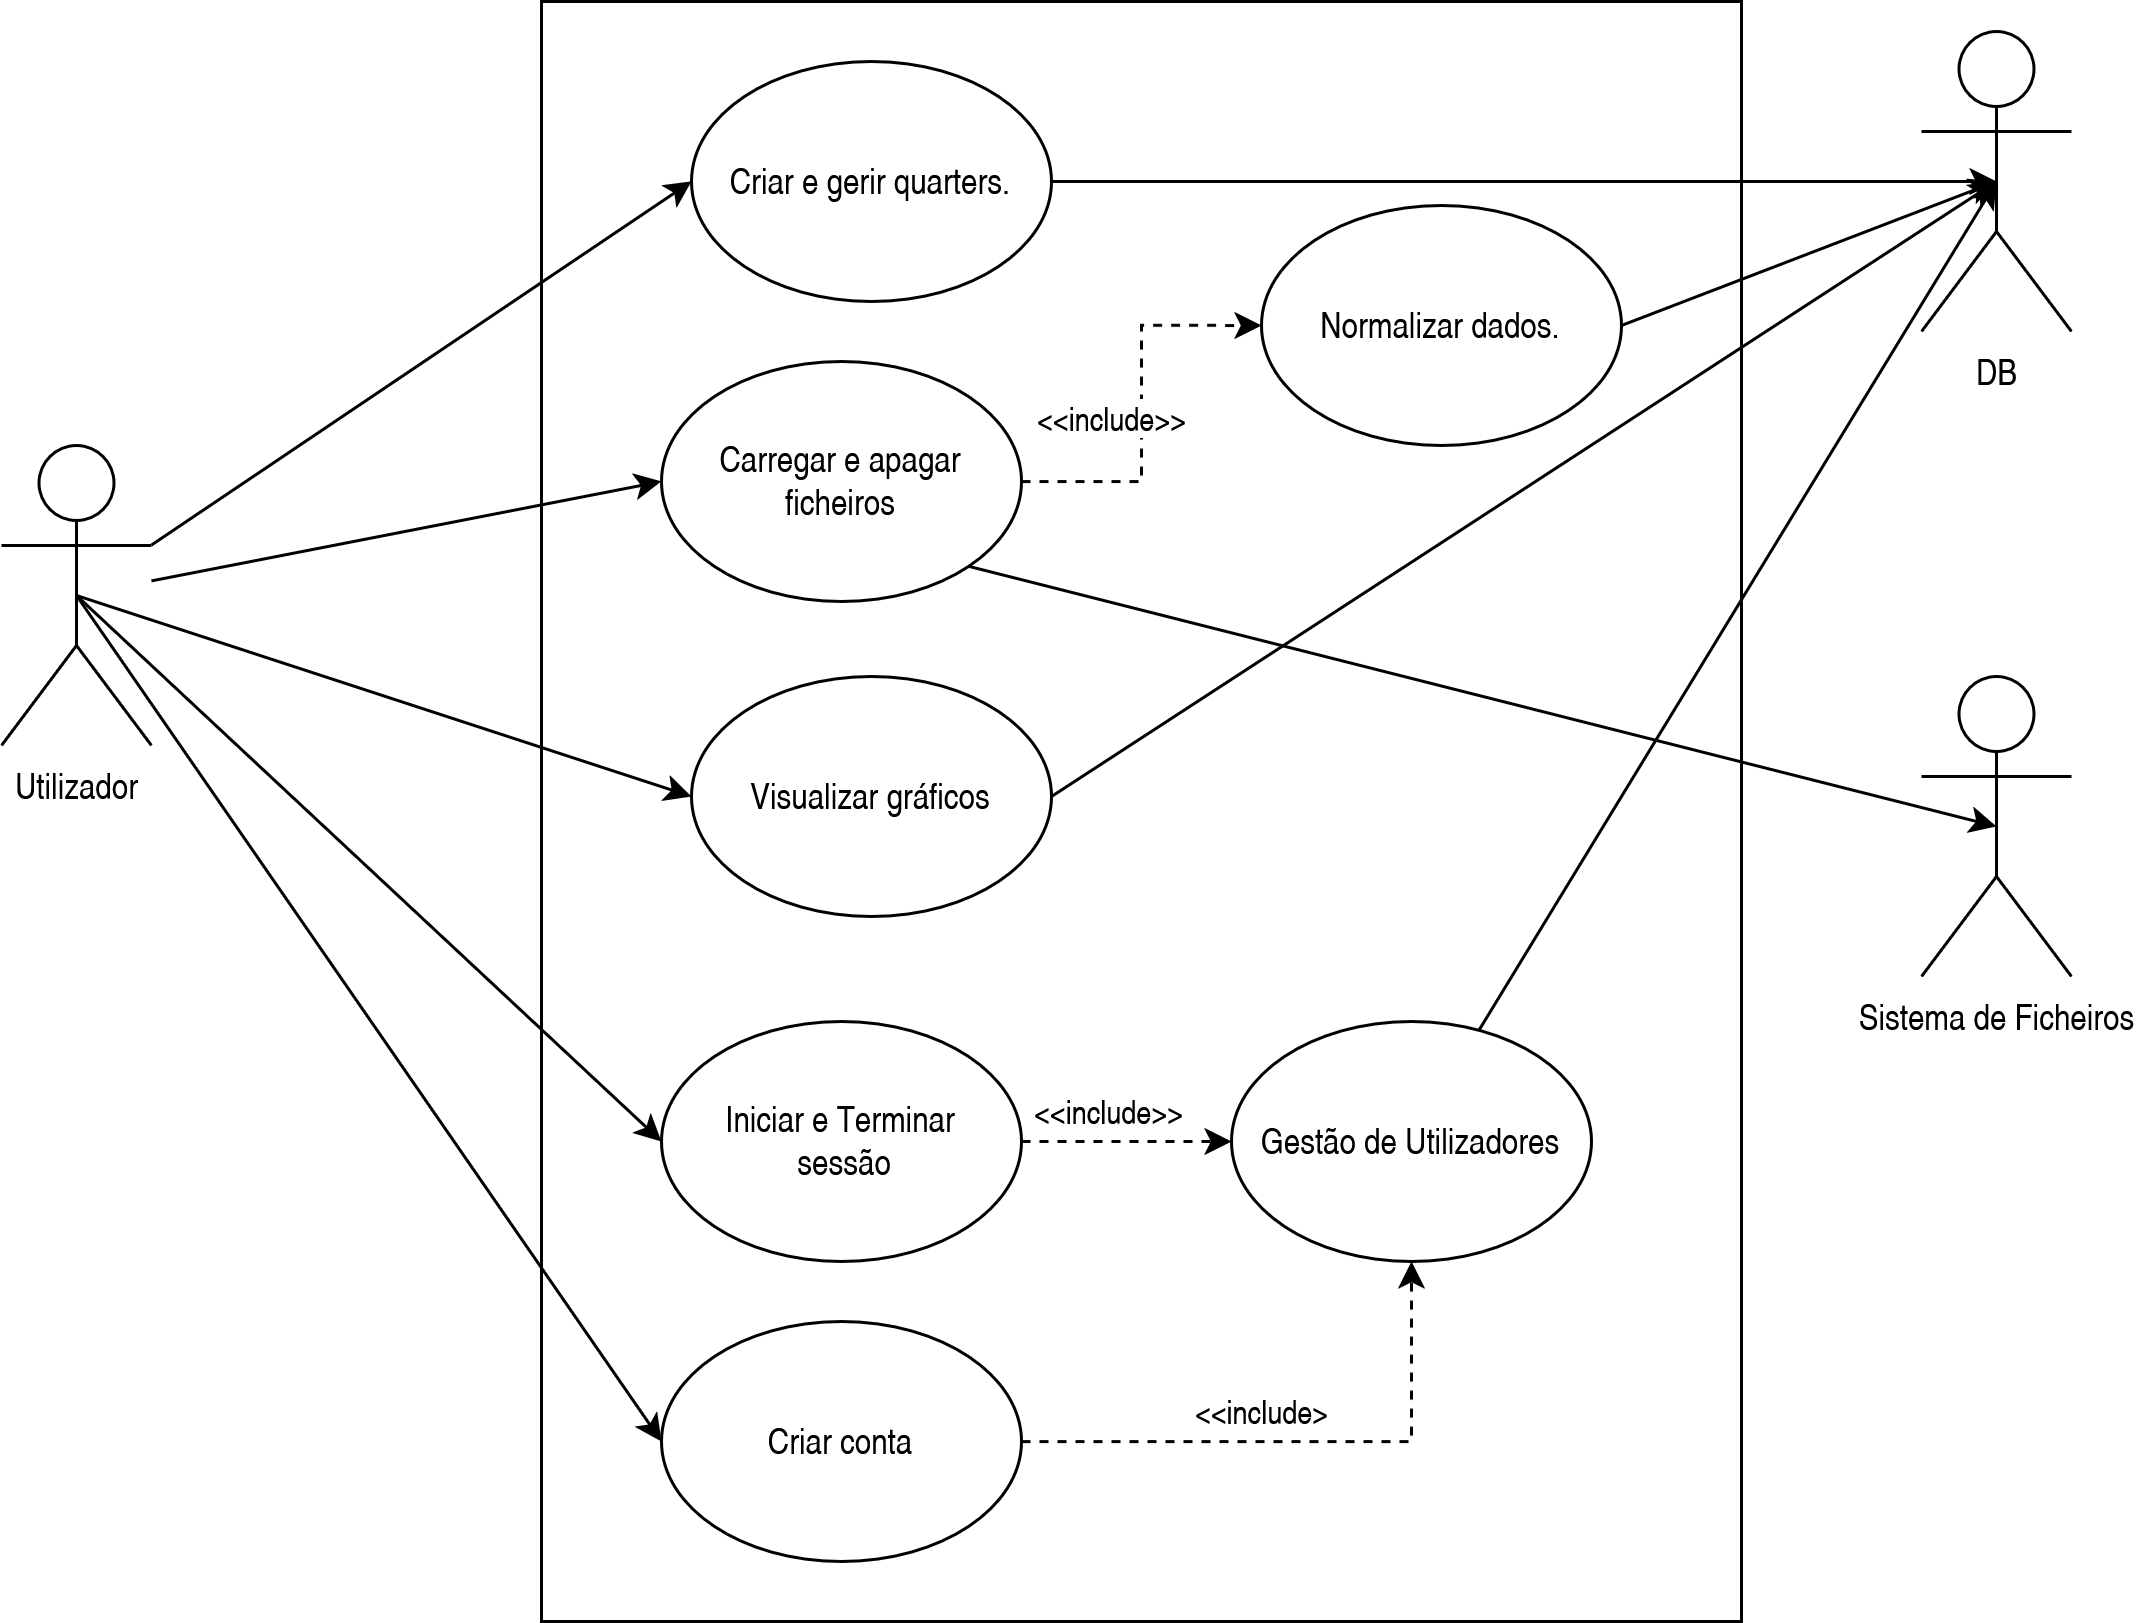
\includegraphics[width=14cm]{./img/usecase_uml}
\caption{\gls{uml} dos Casos de Utilização}
\label{fig:umlCasosUtilizacao}
\end{figure}
\textbf{ Falta a matriz de prioridade dos casos de utilização}


\chapter{Classificação das folhas \gls{xlsx}}


\chapter{Comparação de gráficos suportados pelo Plotly e Chart.js}
\label{ch:charts}

\begin{table}[H]
\centering
\caption{Comparação de tipos de gráficos suportados por Plotly.js e Chart.js}
\begin{tabular}{|l|c|c|}
\hline
\textbf{Tipo de Gráfico} & \textbf{Plotly.js} & \textbf{Chart.js} \\
\hline
Barras                         & Suportado & Suportado \\
Linhas                         & Suportado & Suportado \\
Dispersão (Scatter)            & Suportado & Suportado \\
Circular (Pie)                 & Suportado & Suportado \\
Área                           & Suportado & Suportado \\
Radar                          & Suportado & Suportado \\
Histograma                     & Suportado & Suportado \\
Box Plot                       & Suportado & Não Suportado \\
Mapa de Calor (Heatmap)        & Suportado & Não Suportado \\
Cascata (Waterfall)            & Suportado & Não Suportado \\
Indicadores (Gauges)           & Suportado & Não Suportado \\
Candlestick (Finanças)         & Suportado & Não Suportado \\
OHLC (Finanças)                & Suportado & Não Suportado \\
Treemap                        & Suportado & Não Suportado \\
Sunburst                       & Suportado & Não Suportado \\
Violin                         & Suportado & Não Suportado \\
Mapa (Geo)                     & Suportado & Não Suportado \\
\hline
\end{tabular}
\label{tab:charts}
\end{table}